% !TEX root = ..\Main.tex
\chapter{Zero-Knowledge Proofs and the Ideal Linear Commitment Model}
\label{chapterlabel:Models}

In this chapter, we begin by defining zero-knowledge proofs. Then we define what it means to be an Ideal Linear Commitment protocol, and compare that model with other similar models which give rise to zero-knowledge proof systems.

This chapter is important, as the core contribution of this thesis is to provide efficient Ideal Linear Commitment protocols and show that they can be converted into real proof systems. None of this would be possible without first precisely definining the model.

We choose to present zero-knowledge proofs and the definition of the Ideal Linear Commitment model together in the same chapter, because the two types of protocol will satisfy largely similar security definitions.

\section{Zero-Knowledge Proofs}
\label{shvzkdef}

A \emph{proof system} is defined by a triple of stateful PPT algorithms $(\mathcal{K},\mathcal{P},\mathcal{V})$, which we call the common-reference-string \emph{generator}, the \emph{prover} and \emph{verifier}, respectively.

The setup generator $\mathcal{K}$ creates public parameters $\crs$ which provide the necessary setup information for \prover and \verifier to run the protocol. On input $1^\lambda$, the generator $\crsgen$ produces a common reference string $\crs$. We think of $\crs$ as being honestly generated and use the public parameter model purely for simplicity and efficiency in our proofs. However, in the proofs we construct, $\crs$ consists of parts that are either publicly verifiable or could be generated by the verifier, so we do not rely on the public parameter model for security in any way.

\paragraph{Different Types of Interactive Protocols.} The prover and verifier interact with each other in some sort of \emph{interaction environment}, or \emph{communication channel} which we will denote by $\overset{\textnormal{chan}}{\longleftrightarrow}$. In the usual interaction environment $\std$, all messages are forwarded between prover and verifier. In fact, $\std$ refers to exactly the sort of interaction defined by the complexity class IP. We also consider an \emph{ideal linear commitment} environment, \ILC, defined properly in Section~\ref{formalILCmodel}. This thesis is concerned with producing \ILC\ proof protocols which are defined by interactions between the prover and verifier in the \ILC\ environment.

Why speak of interaction environments at all? We do this because the definitions of what it means to be a secure zero-knowledge proof protocol will really depend very little on whether the interaction takes place as an interactive proof protocol or an \ILC\ protocol. This is to be expected, as \ILC\ proof protocols were designed as an information theoretic abstraction of certain zero-knowledge proofs.

When $\mathcal{P}$ and $\mathcal{V}$ interact on inputs $s$ and $t$ via $\overset{\textnormal{chan}}{\longleftrightarrow}$, then let $\viewV \leftarrow \langle \mathcal{P}(s) \overset{\textnormal{chan}}{\longleftrightarrow} \mathcal{V}(t)\rangle$ be the view of the verifier in the execution, which is made up of all of the verifier's inputs, including random coins, and let $\viewp \leftarrow  \langle \mathcal{P}(s) \overset{\textnormal{chan}}{\longleftrightarrow} \mathcal{V}(t)\rangle$ denote the transcript of the communication between prover and channel. This overloads the notation $\leftarrow  \langle \mathcal{P}(s) \overset{\textnormal{chan}}{\longleftrightarrow} \mathcal{V}(t)\rangle$ but it will always be clear from the variable name if we get the verifier's view or the prover's transcript. At the end of the interaction the verifier accepts or rejects. We write $\langle \mathcal{P}(s)\overset{\textnormal{chan}}{\longleftrightarrow} \mathcal{V}(t)\rangle =b$ depending on whether the verifier rejects ($b=0$) or accepts ($b=1$).

We say a proof system is \emph{public coin} if the verifier's messages to the communication channel are chosen uniformly at random and independently of the actions of the prover, i.e., the verifier's messages to the prover correspond to the verifier's randomness $\rho$. All of our protocols, whether they are \ILC\ protocols, or real protocols compiled under cryptographic assumptions, will be public coin. Public coin protocols are very relevant as they are conceptually simple, and one can prove simpler variants of standard security properties, such as special-honest-verifier zero-knowledge, with the understanding that standard transformations and techniques will provide full security later.

We will model our zero-knowledge proofs using ternary relations $\R$ consisting of tuples $(\crs, \stm,\wit)$. The first item in the tuple is the \emph{common reference string} $\crs$ containing the setup information required for the protocol. Typically, $\crs$ will specify the security parameter $\sep$, perhaps implicitly through its length, and may also contain other parameters used for specifying the specific relation, e.g. a description of a field. Often, $\crs$ will also contain parameters that do not influence membership of $\R$ but may aid the prover and verifier, for instance, a description of an encoding function that they will use. The second item in the tuple, $\stm$ is the \emph{instance} and represents what the prover wants to prove. The final item, $\wit$, is the prover's secret \emph{witness} that $(\crs,\stm)\in\LL_\R$ where the language $\LL_\R \subset \{0,1\}^*$ as follows.
\[ \LL_\R=\{(\crs,\stm)|\exists \wit: (\crs,\stm,\wit)\in \R\} \]
Intuitively speaking, this is the collection of statements which are `true', and for which the verifier should output $1$ after running the protocol with an honest prover. The languages $\LL_\R$ are decidable in polynomial time.

The protocol $(\KK,\mathcal{P},\mathcal{V})$ is called a \emph{proof of knowledge} over communication channel $\overset{\textnormal{chan}}{\longleftrightarrow}$ for relation $\R$ if it has perfect completeness and computational knowledge soundness as defined below.

\begin{definition}[Perfect Completeness]
The proof is \emph{perfectly complete} if for all PPT adversaries $\mathcal{A}$
$$\Pr \left[ \begin{array}{c} \crs\gets \KK(1^\sep); (u,w) \leftarrow \mathcal{A}(\crs): \\
(\crs,u,w)\notin \R ~\vee~ \langle \mathcal{P}(\crs,u,w)\overset{\textnormal{chan}}{\longleftrightarrow}\mathcal{V}(\crs,u)\rangle=1 \end{array}\right] =1.$$
\end{definition}

\begin{definition}[Knowledge soundness]
A public-coin proof system has \emph{computational (strong black-box) knowledge soundness} if for all DPT $\Po^*$ there exists an expected PPT extractor $\E$ such that for all PPT adversaries $\A$
$$\Pr\left[\begin{array}{c} \crs\gets \KK(1^\sep);(\stm,s) \gets \mathcal{A}(\crs); \wit\gets \E^{\langle \Po^*(s)\overset{\textnormal{chan}}{\longleftrightarrow}\V(\crs,\stm)\rangle}(\crs,\stm):\\ b=1 ~\wedge~ (\crs,\stm,\wit)\notin \R \end{array}\right]\approx 0.$$ 
Here the oracle $\langle \Po^*(s)\overset{\textnormal{chan}}{\longleftrightarrow}\V(\crs,\stm)\rangle$ runs a full protocol execution and if the proof is successful it returns a transcript of the prover's communication with the channel. The extractor $\E$ can ask the oracle to rewind the proof to any point in a previous transcript and execute the proof again from this point on with fresh public-coin challenges from the verifier. We define $b\in \{0,1\}$ to be the verifier's output in the first oracle execution, i.e., whether it accepts or not, and we think of $s$ as the state of the prover. The definition can then be paraphrased as saying that if the prover in state $s$ makes a convincing proof, then we can extract a witness.

If the definition holds also for unbounded $\mathcal{P}^*$ and $\A$ we say the proof has {\em statistical knowledge soundness}. 

If the definition of knowledge soundness holds for a non-rewinding extractor, i.e., a single transcript of the prover's communication with the communication channel suffices, we say the proof system has knowledge soundness with {\em straight-line extraction}. 
\end{definition}
\noindent
This definition gives a security guarantee against computationally bounded adversaries. Zero-knowledge protocols satisfying this definition are properly called zero-knowledge arguments of knowledge to distinguish them from zero-knowledge proofs of knowledge, for which knowledge soundness is guaranteed even against unbounded adversaries. However, the term `proofs' is often used in both cases.

\paragraph{Remark.} The definition of knowledge soundness uses a knowledge extractor running in expected polynomial time. One might question the validity of proofs of computational knowledge soundness based on some cryptographic assumption, which prove that either the knowledge extractor extracts a witness, or manages to break some computational assumption in expect polynomial time. This is because cryptographic assumptions are usually defined using probabilistic polynomial time adversaries rather than expected polynomial time adversaries. Fortunately, Markov's inequality allows us to relate the expected polynomial time extractor to a probabilistic polynomial time algorithm. Suppose that the expected running time of the extractor is given by $T$. Then, by Markov's inequality, the probability that the knowledge extractor runs for time longer than $2T$ is at most $1/2$. If we define a new algorithm that runs the knowledge extractor for time at most $2T$ and then aborts if the running time exceeds $2T$, then we have a probabilistic polynomial time algorithm capable of either finding a witness or breaking a computational assumption. This means that it is really possible to reduce the knowledge soundness of the scheme to a standard cryptographic assumption, at the cost of some looseness in the reduction coming from the probability that the knowledge extractor runs for too long and the algorithm aborts.

Another way to define a proof of knowledge follows Groth and Ishai~\cite{GrI08} who borrowed the term witness-extended emulation from Lindell~\cite{Lin03}. Informally, their definition says that given an adversary that produces an acceptable argument with some probability, there exists an emulator that produces a similar argument with the same probability together with a witness $w$. Note that the emulator is allowed to rewind the prover and verifier's interaction to any previous move.

\begin{definition}[Witness-extended emulation]
$(\mathcal{P},\mathcal{V})$ has {\em statistical witness-extended emulation} if for all deterministic polynomial time $\mathcal{P}^*$ there exists an expected polynomial time emulator $\mathcal{E}$ such that for all interactive adversaries $\mathcal{A}$
\begin{align*}
& \Pr \Big{[}(u,s) \leftarrow\mathcal{A}(1^\sep); tr \leftarrow \langle \mathcal{P}^*(u,s)\overset{\textnormal{chan}}{\longleftrightarrow} \mathcal{V}(u)\rangle: \mathcal{A}(tr)=1 \Big{]}\\
\approx \ & \Pr \left[ \begin{array}{l} (u,s) \leftarrow \mathcal{A}(1^\sep); (tr,w) \leftarrow \mathcal{E}^{ \langle \mathcal{P}^*(u,s) \overset{\textnormal{chan}}{\longleftrightarrow} \mathcal{V}(u) \rangle } (u): \\ \mathcal{A}(tr)=1 \text{\emph{ and if }} tr \text{\emph{ is accepting then }} (u,w) \in R \end{array} \right]
\end{align*}
where the oracle called by $\mathcal{E}^{\langle \mathcal{P}^*(u,s), \mathcal{V}(u)\rangle}$ permits rewinding to a specific point and resuming with fresh randomness for the verifier from this point onwards.
\end{definition}
\noindent
Note that in this definition, the role of the adversary $\mathcal{A}$ is as a distinguisher, while it is the job of $\mathcal{P}^*$ to produce proofs. That is why the two are decoupled from one another.

We can interpret $s$ as the state of $\mathcal{P}^*$, including the randomness. So, whenever $\mathcal{P}^*$ is able to make a convincing argument when in state $s$,  $\mathcal{E}$ can extract a witness. Witness Extended Emulation implies Knowledge Soundness \cite{dissertation}.

We will construct public-coin proofs that have special honest-verifier zero-knowledge. This means that if the verifier's challenges are known, or even adversarially chosen, then it is possible to simulate the verifier's view without the witness.  In other words, the simulator works for verifiers who may use adversarial coins in choosing their challenges but they follow the specification of the protocol as an honest verifier would. 
\begin{definition}[Special Honest-Verifier Zero-Knowledge]
The proof of knowledge is \emph{computationally special honest-verifier zero-knowledge (SHVZK)} if there exists a PPT simulator $\mathcal{S}$ such that for all stateful interactive PPT adversaries $\mathcal{A}$ that output $(u,w)$ such that $(\crs,u,w)\in R$ and randomness $\rho$ for the verifier
\begin{eqnarray*}
&&\Pr \left[ \begin{array}{c}\crs\gets \KK(1^\sep);(u, w, \rho) \leftarrow\mathcal{A}(\crs); \\
\viewV\leftarrow \langle \mathcal{P}(\crs,u,w)\overset{\textnormal{chan}}{\longleftrightarrow} \V(\crs,u;\rho)\rangle: \A(\viewV)=1\end{array} \right]\\
&\approx &\Pr \left[ \crs\gets \KK(1^\sep);(u, w, \rho) \leftarrow\mathcal{A}(\crs); \viewV\leftarrow \mathcal{S}(\crs,u,\rho): \mathcal{A}(\viewV)=1\right].
\end{eqnarray*}

We say the proof is \emph{statistically SHVZK} if the definition holds also against unbounded adversaries, and we say the proof is \emph{perfect SHVZK} if the probabilities are exactly equal.
\end{definition}

\section{Introduction to the Ideal Linear Commitment Model}
\label{formalILCmodel}

In this section, we will precisely define Ideal Linear Commitment protocols. We will then compare and contrast this interaction model with other models. Ideal Linear Commitment protocols were first described in \cite{BootleCGGHJ17}, but never completely formally defined. The definitions given in this section are new, and an important contribution of this thesis. Though the definitions are new, they draw inspiration from the definitions of similar models for information-theoretic proof systems, such as Interactive Oracle Proof protocols \cite{Ben-SassonCS16}.

In contrast to standard interactions between a prover and a verifier in IP protocols, we will consider interactions in an \emph{ideal linear commitment} interaction environment, \ILC. Figure~\ref{ILCSyntaxFigure11} provides some graphical insight into how parties in an \ILC\ proof protocol interact. Our motivation for introducing this new interaction environment was to model zero-knowledge proof protocols using compressing and homomorphic cryptographic commitment schemes.

\begin{figure}[htb]
\resizebox{\textwidth}{!}{\begin{tabular}{lll}
$\Po_{\ILC~}$ &\multirow{4}{*}{ \resizebox{0.8\linewidth}{!}{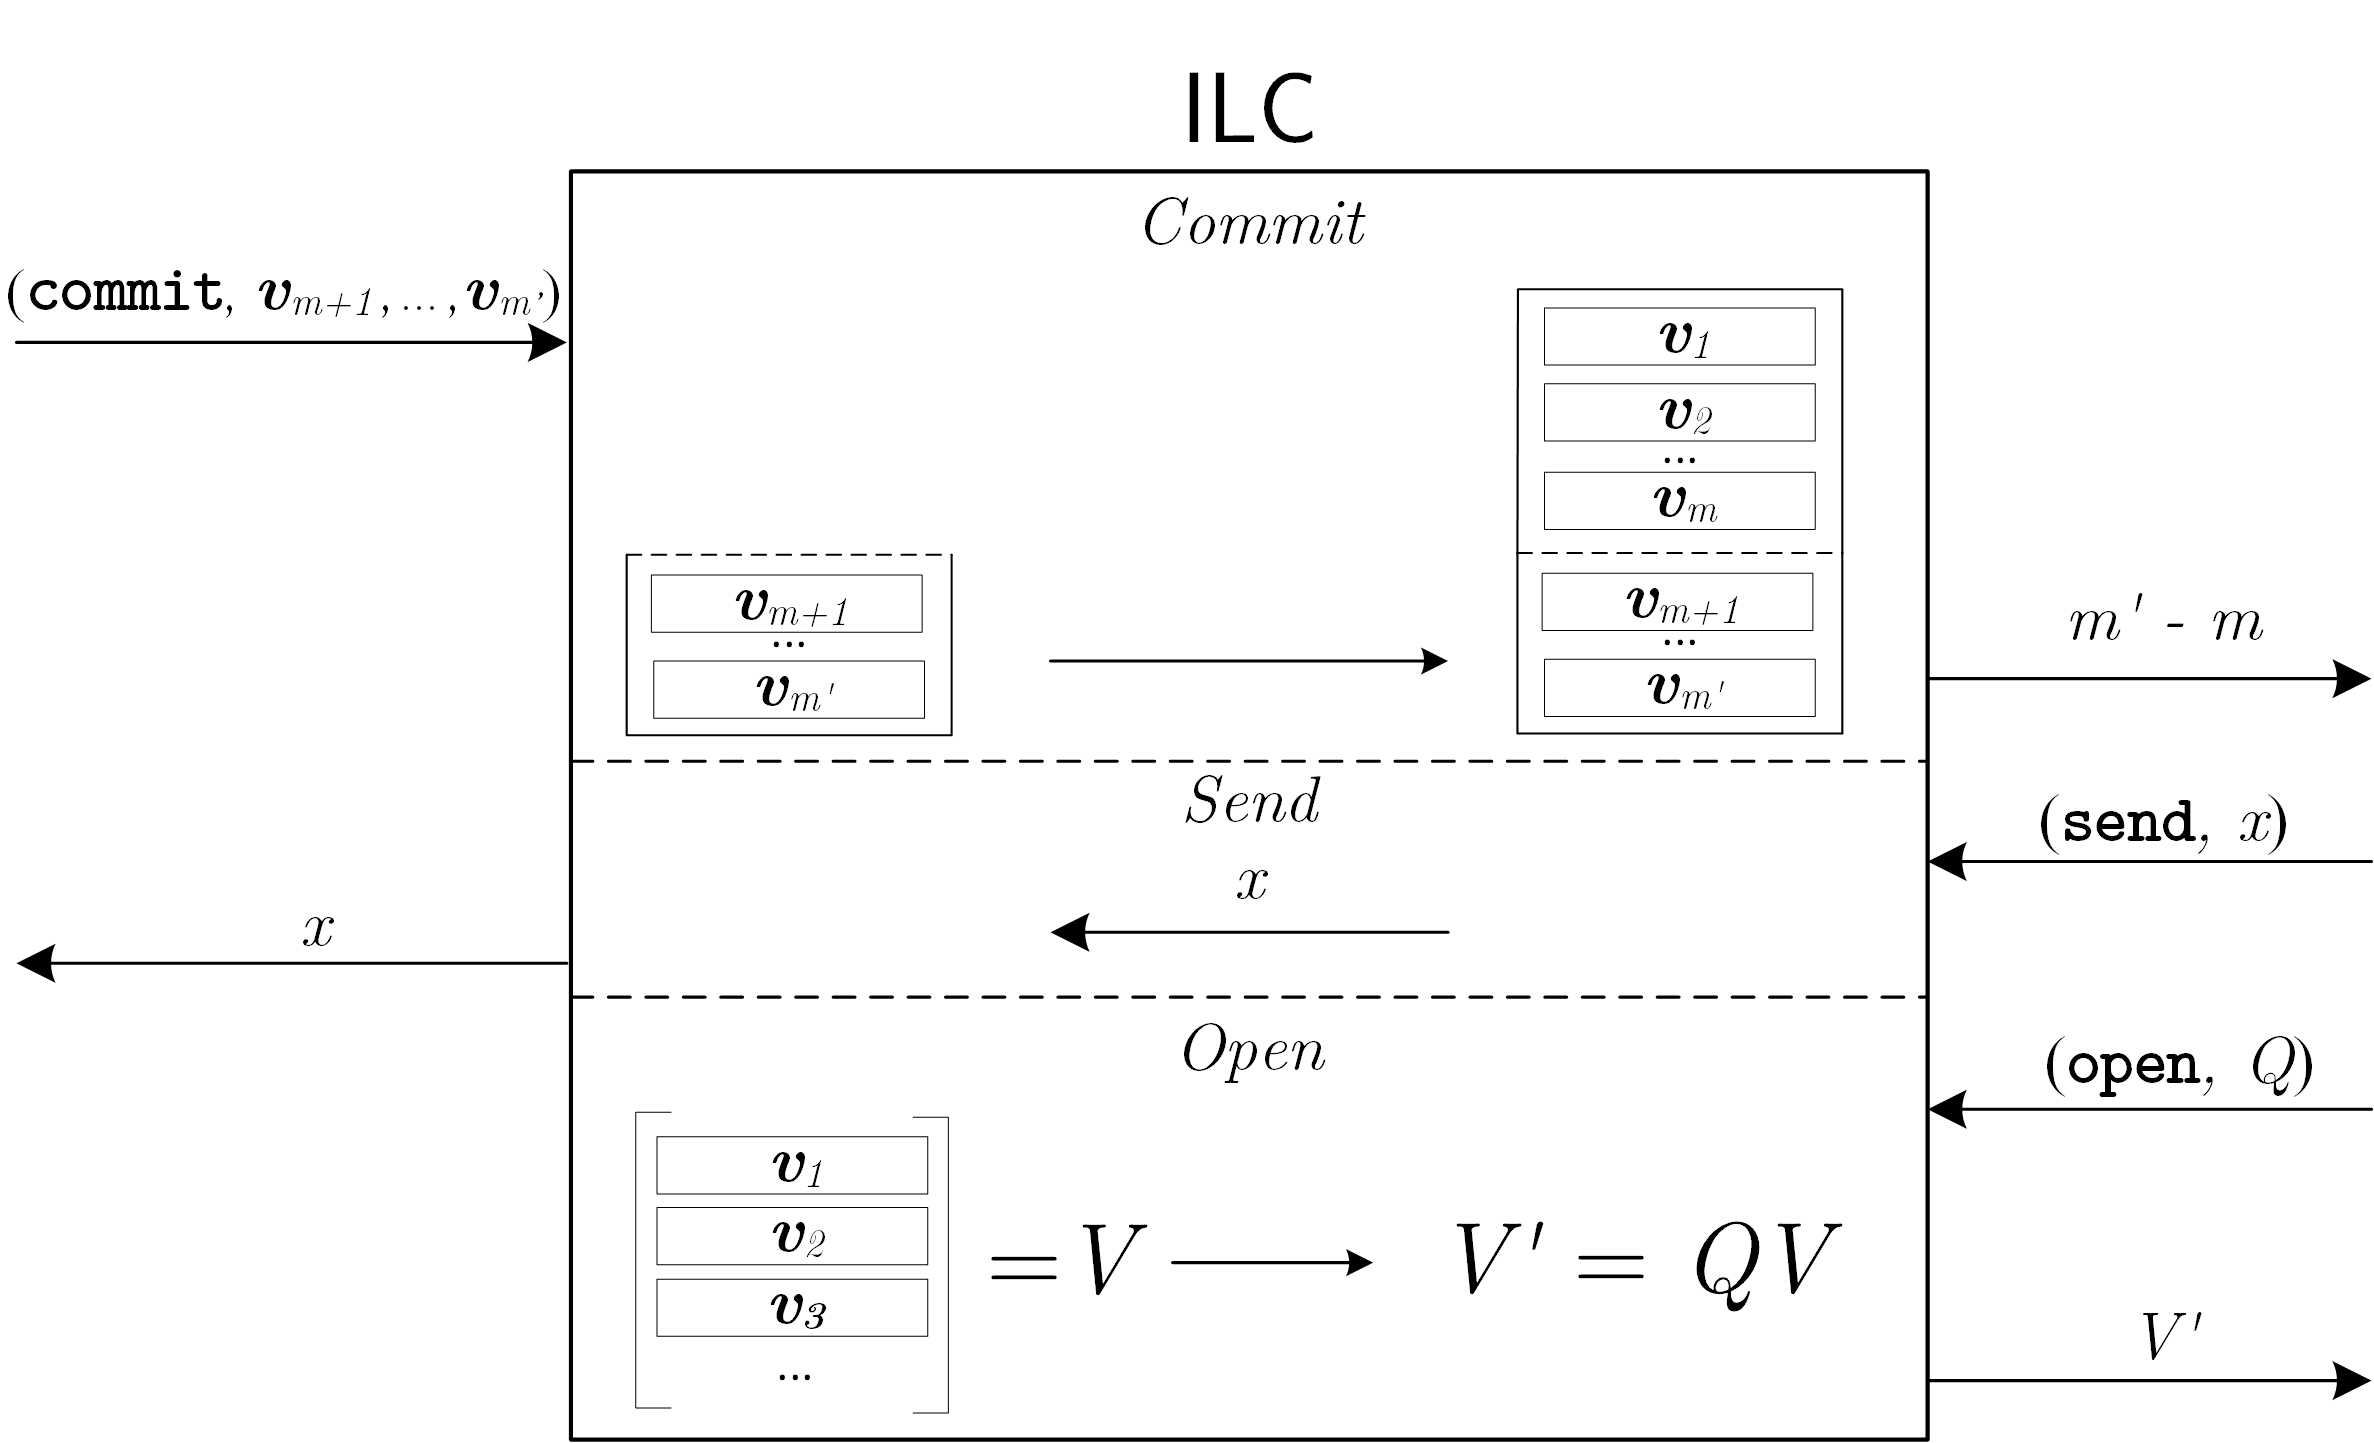
\includegraphics{ILC2-shrink.png}} }&$\V_{\ILC~}$\\
&& \\&&\\&&\\&&\\&&\\&&\\&&\\&&\\&&\\&&\\&&\\
&&\\&&\\
\end{tabular}}\caption{Description of the $\ILC~$ interaction environment. The $\vec{v}_i$ here are vectors over a field $\F$, $x$ is a value from $\F$ and $V, V'$ and $Q$ are matrices over $\F$.}\label{ILCSyntaxFigure11}
\end{figure}

As such, when using the \ILC\ channel, the prover can submit an \ILCcommit\ command to commit to
vectors of field elements of some fixed length $\sizevect$, specified in $\crs_{\ILC}$. The vectors remain secretly stored, and will not be forwarded to the verifier. Instead, the verifier only learns how many vectors the prover has committed to, and their lengths.

The \ILC\ could be viewed in several possible different ways, as a commitment functionality, communication channel, a trusted third party, or an oracle for the verifier. When Ideal Linear Commitment protocols are compiled into real zero-knowledge protocols, the functionality previously guaranteed by the \ILC\ will be enforced using various cryptographic tools.

The verifier can send single field elements to the prover. The original model in \cite{BootleCGGHJ17} described an \ILCsend\ command for this purpose. We removed this command, as we found no need for it when moving to a more precise description of the \ILC\ interaction environment.

The verifier can also submit queries to an \ILCopen\ oracle for obtaining the opening of any linear combinations of the vectors \emph{of the same length} sent by the prover. We stress that the verifier can request several linear combinations within a single \ILCopen\ query, as depicted in Figure~\ref{ILCSyntaxFigure11}.

In addition to the \ILC\ commands and oracles used in the original model \cite{BootleCGGHJ17}, we introduce a new \ILCcheck\ oracle. Inside the \ILC \ model, this command behaves in a very similar way to the \ILCopen\ oracle. However, the two commands will be treated slightly differently when \ILC\ protocols are compiled into real protocols. The reason for making the distinction is that in some of our protocols, the verifier needs to check whether a large vector, that they have computed themselves, is the correct linear combination of vectors committed by the prover. This could be solved by having the verifier make an \ILCsend\ query for the correct linear combination and checking whether the result is equal to the large vector, which incurs a communication cost for the large vector in the \ILC\ protocol. However, in a real protocol, where the verifier's queries will actually be computed and sent by the prover, the verifier can re-commit to the vector that they have computed, and check this against the prover's commitments. In other words, since the verifier has already computed the vector for themself, there is no need for them to receive it again. Therefore, the \ILCcheck\ oracle is used to distinguish this case, which should not be counted as part of the communication costs of a proof. This issue will be discussed further in later chapters.

\subsection{Definitions}

We will now define general Ideal Linear Commitment protocols, and then specialise to the case of public-coin protocols.

\begin{definition}[Ideal Linear Commitment Protocol]

In a $\mu$-round Ideal Linear Commitment protocol, a prover $\PoILC$ and a verifier $\VILC$ will interact with each other via the \ILC, each sending $\mu$ messages. An Ideal Linear Commitment protocol is defined over a field $\F$ and will use a fixed vector length $\sizevect$. Let $(t_1,\ldots,t_\mu) \in \N^\mu$ be a tuple of message lengths. There is a setup generator $\KKILC$ which outputs $\crs_\ILC = (\F,\sizevect,(t_1,\ldots,t_\mu),\mathsf{aux})$, where $\mathsf{aux}$ consists of extra elements of $\F$ which might be useful when running the protocol.

The prover and the verifier will run the protocol on given inputs. They will use random coins $\rho_\Po$ and $\rho_\V$, and they will maintain states $\mathsf{state}^\Po_i$ and $\mathsf{state}^\V_i$ that will allow them to remember information over several different rounds of the protocol. The initial state $\mathsf{state}^\Po_0$ of the prover will be equal to the prover's input. The initial state $\mathsf{state}^\V_0$ of the verifier will be equal to the prover's input. Initially, the \ILC\ will store $V_0$, which is either a matrix with $\sizevect$ columns, or equal to $\bot$. The matrix $V_0$ corresponds to any commitments that have been made before the protocol begins, that might form part of the prover or verifier's input.

In every round $\roundnum \in \{ 1,\ldots,\mu \}$:
\begin{itemize}
\item The prover takes as input the round number $\roundnum$, the setup information $\crs_\ILC$, the verifier's previous messages $m_1,\ldots,m_{\roundnum-1}$, internal state $\mathsf{state}^\Po_{i-1}$, and randomness $\rho_\Po$, and outputs a matrix $V_i \in \F^{t_i \times \sizevect}$ and a new internal state $\mathsf{state}^\Po_{i}$. It commits to $V_i$ using the \ILCcommit\ command.
\item After round $\roundnum$, the \ILC \ stores the vertical concatenation of the matrices $V_0,\ldots,V_\roundnum$.
\item The verifier takes as input the round number $\roundnum$, the setup information $\crs_\ILC$, internal state $\mathsf{state}^\V_{i-1}$, and randomness $\rho_\Po$. It makes linear \ILCopen\ and \ILCcheck\ queries on the contents of the $\ILC$. Then it outputs a new message $m_i \in \F$ and a new internal state $\mathsf{state}_i^\V$.
\item The verifier's final message $m_\mu$ is either $1$, in which case we say the verifier has accepted, or $0$, in which case we say that the verifier has rejected.
\end{itemize}
\end{definition}

We call a proof system over the \ILC\ channel \emph{non-adaptive} if the verifier makes one \emph{open} query and then immediately makes one \emph{check} query to the \ILC\ channel, before terminating his interaction with the channel, and these are the only \emph{open} and \emph{check} queries that the verifier makes. Otherwise we call it \emph{adaptive}. Although adaptive proof systems are allowed, we will only consider non-adaptive \ILC\ proof systems to simplify the exposition. In non-adaptive \ILC\ proof systems with vectors of length $\sizevect$, the verifier will produce two query matrices, $Q$ for the \ILCopen\ query and $Q'$ for the \ILCcheck\ query. 

We give pseudocode descriptions of an Ideal Linear Commitment protocol in Figure \ref{fig:ILCpseudocode}. Here, $\VILC^{\ILCopen(\cdot),\ILCcheck(\cdot,\cdot)}$ means that $\VILC$ has access to \ILCopen\ and \ILCcheck\ oracles.

\begin{figure}[!h]
\resizebox{\textwidth}{!}{
\begin{minipage}[t]{13cm}
\begin{algorithm}[H]
\caption*{An \ILC\ Protocol on $\crs_\ILC,\rho_\Po,\rho_\V,\mathsf{state}_0^\Po, \mathsf{state}_0^\V$ }
\begin{itemize} \item\textbf{Initialise protocol.}:
\begin{itemize}
\item Set $M = V_0$.
\end{itemize} 
\item \textbf{For $i = 1$ to $\mu$}: 
\item \qquad \textbf{Run prover algorithm}:
\begin{itemize}
\item $(V_i,\mathsf{state}^\Po_i) \gets \Po_\ILC ( i, \lbrace m_j \rbrace_{j < i}, \mathsf{state}^\Po_{i-1}, \rho_\Po )$
\item $\ILCcommit(V_i)$
\end{itemize}
\item \qquad \textbf{Run verifier algorithm}:
\begin{itemize}
\item $(m_i,\mathsf{state}_i^\V) \gets \VILC^{\ILCopen(\cdot),\ILCcheck(\cdot,\cdot)}(i,\mathsf{state}^\V_{i-1},\rho_\V)$
\end{itemize} 
\item \textbf{Accept or Reject}
\end{itemize} 
\vspace{1.53cm}
\end{algorithm}
\end{minipage}
%==============================================================
\begin{minipage}[t]{6.5cm}
\vspace{0cm}
\begin{algorithm}[H]
\caption*{\ILCcommit($V$)}
\begin{itemize}
\item If $M = \bot$ then set $M = V$.
\item If $V = \bot$ then do nothing.
\item Otherwise, update $M$ by vertically concatenating it with $V$, with $V$ at the bottom.
\end{itemize}
\end{algorithm}
%\vspace{-1.07cm}
\begin{algorithm}[H]
\caption*{\ILCopen($Q$)}
\begin{itemize}
\item Output $QM$.
\end{itemize}
\end{algorithm}
%\vspace{-1.07cm}
\begin{algorithm}[H]
\caption*{\ILCcheck($Q', V'$)}
\begin{itemize}
\item If $Q'M = V'$ then output $\top$.
\item Otherwise output $\bot$.
\end{itemize}
\end{algorithm}
%\vspace{0.1cm}
\end{minipage}
}
\caption{Description of how the parties in an \ILC\ protocol interact.}
%For explanation, see Subsection~\ref{ssec:constrILCtoIOP}}
\label{fig:ILCpseudocode}
\end{figure}

The security properties of \ILC\ proof protocols, including the completeness, soundness, and zero-knowledge properties, are defined in exactly the same way as for normal zero-knowledge protocols.

\subsection{Complexity Measures}

We have already mentioned $\mu$, the number of rounds of an \ILC\ protocol. This is our first useful complexity measure.

W also consider is $t = \sum_{i=1}^\mu t_i$. This is the \emph{total number of vectors} that the prover commits to as part of the \ILC\ protocol. Later one, we will see that this can impact the communication complexity and computational complexity of real protocols based on \ILC\ protocols.

We define $\qc$ to be the \ILCopen\ query complexity, i.e. the number of times that the verifier uses the \ILCopen\ oracle. Similarly, we define $\qc'$ to be the \ILCcheck\ query complexity, i.e. the number of times that the verifier uses the \ILCcheck\ oracle. 

%We define $\qc$ to be the \ILCopen\ query complexity, i.e., $\Chal \in \F^{\qc\times t}$, and $\qc'$ the \ILCcheck\ query complexity, i.e., $\Chal' \in \F^{\qc'\times t}$. Let $T_{\PoILC}$ be the running time of $\PoILC(\crs_{\ILC},\stm,\wit)$, $T_{\ECC\!}(\sizevect)$ be the encoding time for a vector in $\F^\sizevect$, $T_{\ComCommit}(t_\roundnum)$ be the time to commit to $t_\roundnum$ field elements, $T_{\text{Mmul}}(\qc,\totalnumvec,b)$ be the time it takes to multiply matrices in $\F^{\qc\times \totalnumvec}$ and $\F^{\totalnumvec\times b}$ and similarly for $\qc'$. Let $T_{\VILC}$ be the running time of $\VILC(\crs_{\ILC},\stm)$, and let $C_{\ILC}$ be the communication from the verifier to the prover in $\langle \PoILC \ilc \VILC\rangle$, $C_{\ComCommit}(t_\roundnum)$ be the combined size of commitment and randomness for a message consisting of $t_\roundnum$ field elements.

Following \cite{BonehBCGI19}, we define the \emph{degree} of an \ILC\ verifier.

\begin{definition}[Degree of \ILC\ Verifier]
We say that an \ILC\ protocol has a degree $d$ verifier if the following hold.
\begin{itemize}
\item The verifier's output state $\mathsf{state}_i^\V$ is a vector in $\F^{w_i}$.
\item There exists a check polynomial $T \ : \ \F^{\sum_{i=1}^\mu w_i + \qc \cdot \sizevect} \to \F^{qc' \times \sizevect}$ of degree $d$ that takes as input the verifier's state at each round of the protocol and the verifier's \ILCopen\ queries, and outputs the matrices $V'$ for the verifier's \ILCcheck\ queries.
\item The verifier accepts if and only if the result of the check query is $\top$.
\end{itemize}
\end{definition}

\subsection{Public Coin Protocols}

As with zero-knowledge protocols, we say that an Ideal Linear Commitment protocol is \emph{public coin} if the following conditions hold.
\begin{enumerate}
\item \emph{Except for the final message} $m_\mu$, the verifier's messages to the communication channel are chosen uniformly at random from $\F$ and independently of the actions of the prover, i.e., the verifier's messages $m_i$ correspond to the verifier's randomness $\rho_\V$.
\item The query matrices $\Chal$ and $\Chal'$ in the verifier's \ILCopen\ and \ILCcheck\ queries are determined only by the values of $m_1,\ldots,m_\roundnum$ that have appeared in the protocol so far. The query matrices $\V'$ in the verifier's \ILCcheck\ queries are determined only by the values of $m_1,\ldots,m_\roundnum$ that have appeared in the protocol so far and by the values of \ILCopen\ query responses that the verifier has seen for far. In particular, this means that the prover can actually antipicate the queries that will be made, because the verifier never uses information that the prover doesn't know when making queries.
\item The verifier's final message $m_\mu$ is determined by the messages $m_1,\ldots,m_{\mu-1}$ and the results of the queries made so far.
\end{enumerate}
%
In this case, we are able to make several simplifications. Since for $i < \mu$ the verifier's messages $m_i$ only depend on $\rho_\V$, all \ILCopen\ and \ILCcheck\ queries can be deferred until the end of the protocol, since they will not affect the messages in any way. In fact, the verifier will only need to make one \ILCopen\ query and then one \ILCcheck\ query. Similarly, the state of the verifier will not affect any of the messages $m_i$ for $i < \mu$, so the verifier need not update state their state either, apart from possibly producing a final state $\mathsf{state}^\V_\mu$ after making the \ILCopen\ and \ILCcheck\ queries.

%We can separate the verifier into three functions. These are the following:
%\begin{itemize}
%\item Query algorithm $Q(m_1,\ldots,m_{\mu-1})$ which computes the matrices $Q$ and $Q'$ for the verifier's \ILCopen\ and \ILCcheck\ queries.
%\item Check algorithm $V' = T(V^*,m_1,\ldots,m_{\mu-1})$ which given the previous messages and the result $V*$ of the \ILCopen queries, computes the matrix $V'$ for the verifier's \ILCcheck\ queries.
%\item Decision algorithm $m_\mu = D(V^*,b,m_1,\ldots,m_\mu)$ which takes the results $V^*$ and $b$ of the \ILCopen\ and \ILCcheck\ queries and the verifier's previous messages, and decides whether to accept or reject.
%\end{itemize}
%
%We give a description of a public-coin \ILC\ protocol in Figure \ref{fig:ILCpseudocode2}.
%
%In the case that a protocol is public-coin and has a verifier of degree $d \in \N$ at the same time, protocols are particularly simple, because the check algorithm is a polynomial, and the decision algorithm simply sets $m_\mu = b$, the result of the \ILCcheck\ query. All of our \ILC\ protocols will be of this form.
%
%\begin{figure}[!h]
%\resizebox{\textwidth}{!}{
%\begin{minipage}[t]{13cm}
%\begin{algorithm}[H]
%\caption*{A public coin \ILC\ Protocol on $\crs_\ILC,\rho_\Po,\rho_\V,\mathsf{state}_0^\Po, \mathsf{state}_0^\V$ }
%\begin{itemize} \item\textbf{Initialise protocol.}:
%\begin{itemize}
%\item Set $M = V_0$.
%\end{itemize} 
%\item \textbf{For $i = 1$ to $\mu-1$}: 
%\item \qquad \textbf{Run prover algorithm}:
%\begin{itemize}
%\item $(V_i,\mathsf{state}^\Po_i) \gets \Po_\ILC ( i, \lbrace m_j \rbrace_{j < i}, \mathsf{state}^\Po_{i-1}, \rho_\Po )$
%\item $\ILCcommit(V_i)$
%\end{itemize}
%\item \qquad \textbf{Select verifier's message}:
%\begin{itemize}
%\item $m_i \gets_{\rho_\V} \F$
%\end{itemize}
%\item \textbf{Run prover algorithm}:
%\begin{itemize}
%\item $(V_\mu,\mathsf{state}^\Po_\mu) \gets \Po_\ILC ( \mu, \lbrace m_j \rbrace_{j < \mu}, \mathsf{state}^\Po_{\mu-1}, \rho_\Po )$
%\item $\ILCcommit(V_\mu)$
%\end{itemize}
%\item \textbf{Run verifier algorithm}:
%\begin{itemize}
%\item $(Q,Q') = Q(m_1,\ldots,m_{\mu-1})$.
%\item $V^* = \ILCopen(Q)$
%\item $V' = T(V^*,m_1,\ldots,m_{\mu-1})$
%\item $b = \ILCcheck(Q',V')$
%\item $m_\mu \gets D(V^*,b,m_1,\ldots,m_\mu)$
%\end{itemize} 
%\item \textbf{Accept or Reject}
%\end{itemize} 
%\vspace{1.53cm}
%\end{algorithm}
%\end{minipage}
%==============================================================
%\begin{minipage}[t]{6.5cm}
%\vspace{0cm}
%\begin{algorithm}[H]
%\caption*{\ILCcommit($V$)}
%\begin{itemize}
%\item If $M = \bot$ then set $M = V$.
%\item If $M = \bot$ then set $M = V$.
%\item Otherwise, update $M$ by vertically concatenating it with $V$, with $V$ at the bottom.
%\end{itemize}
%\end{algorithm}
%\vspace{-1.07cm}
%\begin{algorithm}[H]
%\caption*{\ILCopen($Q$)}
%\begin{itemize}
%\item Output $QV$.
%\end{itemize}
%\end{algorithm}
%\vspace{-1.07cm}
%\begin{algorithm}[H]
%\caption*{\ILCcheck($Q', V'$)}
%\begin{itemize}
%\item If $Q'V = V'$ then output $\top$.
%\item Otherwise output $\bot$.
%\end{itemize}
%\end{algorithm}
%\vspace{0.1cm}
%\end{minipage}
%}
%\caption{Description of how the parties in a public-coin \ILC\ protocol interact.}
%For explanation, see Subsection~\ref{ssec:constrILCtoIOP}}
%\label{fig:ILCpseudocode2}
%\end{figure}

\subsection{Remarks on the Interaction Model}

\paragraph{Remark.} We have presented an interaction environment using vectors of fixed length $\sizevect$. In fact, in our protocols, we will allow the prover to commit to vectors of \emph{several different fixed lengths} $\sizevect_1,\ldots,\sizevect_r$, which will be specified at the beginning of the protocol. This is easily formalised by defining a new interaction environment, giving the prover and verifier access to $r$ copies of different \ILCcommit, \ILCopen\ and \ILCcheck\ commands and oracles using vectors of lengths $\sizevect_1,\ldots,\sizevect_r$. Such a channel will be referred to as an \ILC\ channel for vectors of several fixed lengths, and will be specified simply by including multiple vector lengths in $\crs_{\ILC~}$ rather than just one. The resulting interaction environment is shown in Figure \ref{fig:ILCpseudocodemixlen}.

Alternatively, we can easily incorporate vectors of different lengths into the model by padding all vectors with zeroes until they are the same length as the longest vector. This will have no impact on the asymptotic efficiency of our protocols. Some of our \ILC\ protocols require single values to be committed as well as vectors. 

\begin{figure}[!h]
\resizebox{\textwidth}{!}{
\begin{minipage}[t]{13cm}
\begin{algorithm}[H]
\caption*{An \ILC\ Protocol on $\crs_\ILC,\rho_\Po,\rho_\V,\mathsf{state}_0^\Po, \mathsf{state}_0^\V$ }
\begin{itemize} \item\textbf{Initialise protocol.}:
\begin{itemize}
\item Parse $\crs_\ILC = (\F,\sizevect_1,\ldots,\sizevect_r)$.
\item Set $M_j = V_{0,j}$ for each $j \in [r]$.
\end{itemize} 
\item \textbf{For $i = 1$ to $\mu$}: 
\item \qquad \textbf{Run prover algorithm}:
\begin{itemize}
\item $(V_{i,1},\ldots,V_{i,r},\mathsf{state}^\Po_i) \gets \Po_\ILC ( i, \lbrace m_j \rbrace_{j < i}, \mathsf{state}^\Po_{i-1}, \rho_\Po )$
\item $\ILCcommit(\sizevect_j,V_{i,j})$ for each $j \in [r]$.
\end{itemize}
\item \qquad \textbf{Run verifier algorithm}:
\begin{itemize}
\item $(m_i,\mathsf{state}_i^\V) \gets \VILC^{\ILCopen(\cdot,\cdot),\ILCcheck(\cdot,\cdot,\cdot)}(i,\mathsf{state}^\V_{i-1},\rho_\V)$
\end{itemize} 
\item \textbf{Accept or Reject}
\end{itemize} 
\vspace{1.53cm}
\end{algorithm}
\end{minipage}
%==============================================================
\begin{minipage}[t]{6.5cm}
\vspace{0cm}
\begin{algorithm}[H]
\caption*{\ILCcommit($\sizevect_i,V$)}
\begin{itemize}
\item If $M_i = \bot$ then set $M_i = V$.
\item If $V = \bot$ then do nothing.
\item Otherwise, update $M_i$ by vertically concatenating it with $V$, with $V$ at the bottom.
\end{itemize}
\end{algorithm}
%\vspace{-1.07cm}
\begin{algorithm}[H]
\caption*{\ILCopen($\sizevect_i,Q$)}
\begin{itemize}
\item Output $QM_i$.
\end{itemize}
\end{algorithm}
%\vspace{-1.07cm}
\begin{algorithm}[H]
\caption*{\ILCcheck($\sizevect_i,Q', V'$)}
\begin{itemize}
\item If $Q'M_i = V'$ then output $\top$.
\item Otherwise output $\bot$.
\end{itemize}
\end{algorithm}
%\vspace{0.1cm}
\end{minipage}
}
\caption{Description of how the parties in an \ILC\ protocol with several vector lengths interact.}
%For explanation, see Subsection~\ref{ssec:constrILCtoIOP}}
\label{fig:ILCpseudocodemixlen}
\end{figure}

\paragraph{Remark.} It is of course easy to generalise to the case where the verifier's messages are not single field elements. We use the case of single field elements for notational simplicity and because it suffices for all of our protocols.

\paragraph{Remark.} We will assume that all parties output messages which parse correctly. In other words, no party or functionality will ever deviate from the protocol using messages which are from the wrong domain, or of incorrect length. This will not be a problem for security. Indeed, provided that checking the format of a message can be done efficiently, it would be simple, but tedious, to add such checks at the beginning of every algorithm, and instruct all algorithms to abort if the checks are failed. We assume that this is the case in all of our compiled protocols.

\paragraph{Remark.} If we had followed the original model of \cite{BootleCGGHJ17}, we might have allowed sequences of \ILCcommit, \ILCsend\ and \ILCopen\ and \ILCcheck\ queries to be performed in an arbitrary order. Our definition does not incur a loss in generality by having the prover and verifier alternate in the protocol, as valid protocols in the original model could be recovered by having rounds in which either the prover does nothing or the verifier does not use certain oracles. Rather, our definition corresponds to a sensible reordering of such protocols. For example, the verifier gains no power by being able to make an \ILCopen\ query directly after sending a message to the prover, but before the prover has committed to any new vectors. The verifier might just as well compute their message without sending it, make their query, and then send the message.

\paragraph{Remark.} The verifier also produces a state in their final round, in addition to their final message $m_\mu \in \lbrace 0,1 \rbrace$ which signifies whether they want to accept or reject. This serves a useful purpose. In Section \ref{subsec:polycommit}, we define a polynomial commitment scheme in the \ILC\ model. At the end of the protocol, the verifier is able to compute the evaluation of a committed polynomial and then store it in their final state. In this way, the polynomial commitment scheme can be used as a subprotocol in other \ILC\ protocols, as the evaluation can be passed around as part of the final state.

\subsection{Comparison with Other Models and Types of Protocol}

\paragraph{Interactive Oracle Proofs.} Interactive Oracle Proofs (IOPs) were introduced in \cite{Ben-SassonCS16}. They were designed to simultaneously generalise the interactive protocols of the class IP and probabilistically-checkable proofs (PCPs). IOP protocols share a similar syntax and pattern of interaction to \ILC\ protocols, but the most significant difference is in the verifier's query oracles. In IOP protocols, the prover sends functions to the verifier, and the verifier may make queries to learn the values of these functions at certain points. If one views a function as a long string which is the concatenation of all possible outputs of the function, then one can imagine the verifier making pointwise queries on the string. This naturally leads to the idea of instantiating IOP protocols using commitments based on Merkle trees \cite{Ben-SassonBHR18} which can be efficiently opened to individual positions of a committed string.

Thus, the key difference between IOP and \ILC\ protocols is that IOP protocols use \emph{pointwise} queries rather than linear queries. This difference leads to another difference in the interaction environment. In IOP protocols, the prover commits to a different function or string in each round, and the verifier has separate oracle access to each string committed so far. On the other hand, the \ILC\ stores a matrix $M$ which is updated using the prover's \ILCcommit\ commands, accumulating all committed vectors into a single matrix which the verifier can make queries on, rather than allowing the verifier to make queries on each matrix separately. This clearly leads to more powerful protocols when linear queries are involved; as the verifier can, for example, make a query and obtain a vector $\vec{a}x+\vec{b}$, where $\vec{a}$ and $\vec{b}$ are from different committed matrices, without learning the value of either $\vec{a}$ or $\vec{b}$.

\paragraph{Linear Interactive Proofs.} Linear Interactive Proofs  (LIPs) were introduced in \cite{BitanskyCIPO13}. In linear interactive proofs both the prover and verifier send vectors of field elements, but the prover can only send linear (or affine) transformations of the verifier's previously sent vectors. This is a good model for certain types of zero-knowledge protocol which use a trusted setup. In such cases, the trusted setup consists of various messages, encoded, for example, inside elements from a finite group or suitable homomorphic encryption scheme or commitment scheme. The prover can manipulate the messages in a linear fashion, via the group elements or ciphertexts, but cannot produce new encodings by any other method. An example of a zero-knowledge proof that can be modelled in this way is given in \cite{Gennaro2013}.

Both models use vectors of fixed lengths over fields. However, for LIPs, it is the prover who is restricted to certain types of linear computations, as the inspiration for this model came from proofs where the \emph{prover} manipulates homomorphic commitments. For our constructions it is important that the prover can compute on field elements received by the verifier and for instance evaluate polynomials, while it is the \emph{verifier} who is restricted to linear queries, as the inspiration for our model came from proofs where the verifier manipulates homomorphic commitments.

\paragraph{(Fully) Linear PCPs and (Fully) Linear IOPs}

Linear PCPs were introduced in \cite{BitanskyCIPO13} as a further abstraction of arguments lying behind some LIPs. They were generalised to fully-linear PCPs in \cite{BonehBCGI19}. Just as PCPs were generalised by IOPs, the same paper, \cite{BonehBCGI19} goes on to generalise LPCPs further to (fully-)linear IOPs.

All of these formal models are very closely related to the \ILC\ model. In these models, the prover produces proof strings defined over some field, and the verifier is allowed to make linear queries on the proof strings. The prover produces one proof string in an LPCP protocol, whereas in a LIOP protocol, the prover produces several proof strings over several rounds of interaction with the verifier. In the fully-linear case, the verifier is further restricted so that in addition, they can only make linear queries on the instance $\stm$.

The differences between \ILC\ protocols and LIOP protocols are largely motivated by different efficiency metrics. Intuitively, a LIOP protocol behaves like an \ILC\ protocol where the fixed vector length $\sizevect$ is equal to $1$, and both types of protocol can be converted into the other, although the resulting protocols may suffer unusual parameter choices. For example, an \ILC\ protocol with $\sizevect = 1$ is possible, but when converted into a real protocol using a highly-compressing homomorphic commitment scheme, it is easy to imagine that we create a more efficient protocol by committing to more than one element at once.

LPCP and LIOP protocols are suitable for modelling zero-knowledge proofs where the prover uses non-compressing methods to hide their messages, perfectly binding homomorphic commitment schemes, or homomorphic encryption schemes. The `fully-linear' abstraction captures the case where the instance $\stm$ also relates to encrypted or committed data, for example, and the prover wishes to give a proof about the data.